\chapter{Luminescent Organic Materials}
\label{chapter: luminscent organic materials}
%%%%%%%%%%%%%%%%%%%%%%%%%%%%%%
\section{Introduction}\label{section: lom introduction}
Luminescent organic molecules have myriad of useful applications. In aqueous solution they are used extensively in biological imaging, probing, and detection. Deposited as thin films and aggregates, they represent the next generation of organic optoelectronics, where availability and low cost of starting materials, straightforward syntheses, and lightweight devices are attractive features. Perhaps most importantly, the luminescent response of molecular organic systems can be tuned with relative ease compared to their inorganic counterparts, emitting across the visible spectrum and producing white light. 

Since the discovery of electromluminescence in the 1960s, intensive efforts in academia and industry have delivered considerable progress in the field of organic electronics, leading to  the development of applications such as field-effect transistors, photovoltaic cells, optical memory devices, and single-crystal lasers.\cite{Ostroverkhova2016} The most prominent success story is certainly organic light-emitting diodes (OLEDs), which have already reached market adoption for lighting and display purposes. However, in many areas organic systems suffer from low efficiencies, trial-and-error optimisation, and decreased performance in aggregated form versus solution. 

To advance, there must be control over both the supermolecular structure of the material and the electronic structure of the  molecules within.  Unfortunately neither of these properties exist in isolation, and the interplay between them must also be intimately understood, which somewhat complicates matters. Of these three contributing factors, it is the relationship between the electronic structure and the environment which are of interest in this work. The luminescent response of molecules can change drastically from one medium to another, whether in the gas phase, as a solution, aggregated as clusters, or in molecular crystals. Understanding the interplay between the luminophore and its environment is crucial for designing more efficient materials from first principles. 

To this end, we approach this problem using theoretical chemistry methods to investigate organic compounds exhibiting aggregation induced emission (AIE).  AIE-active compounds are non-emissive in dispersed media, but undergo a switch-on of luminescence, typically in the form of fluorescence, upon aggregation. Since organic electronics are manufactured using a solid-state layer, AIE has attracted considerable interest as a pathway to overcome the common effect of aggregation caused quenching (ACQ), hitherto a major obstacle in the development of organic luminophores. In this chapter the problem of ACQ shall be introduced, followed by an examination of the AIE phenomenon through analysis of typical structures, mechanistic interpretations, and how quantum chemical methods are applied to model such systems.
%%%%%%%%%%%%%%%%%%%%%%%%%%%%%%
\section{Aggregation Caused Quenching}\label{section: lom ACQ}
Photoinduced luminescence occurs after chromophores with $\pi$-conjugation, typically in the form of aromatic moeities, absorb light in the UV/Vis region of the electromagnetic spectrum. In good solvents or dilute concentration, fluorescence usually follows. Upon aggregation with increased concentration, or crystallisation, the fluorescence is often reduced or quenched completely. In 1954, photochemisty pioneer  F\"{o}rster elegantly showed that the fluorescence of pyrene is shifted and weakened with increasing concentration (Figure \ref{figure: Forster_Spectra}).\cite{Forster1954,Forster1969} As the concentration increases, a new fluorescent species is formed and the monomer fluorescence is decreased. The new band at lower energy is a result of the formation of excited dimers, or \textit{excimers}. The presence of aromatic rings in conventional luminophores leads to intermolecular $\pi$-$\pi$ interactions and the formation of excimers. 
\begin{figure}[H]
\centering
  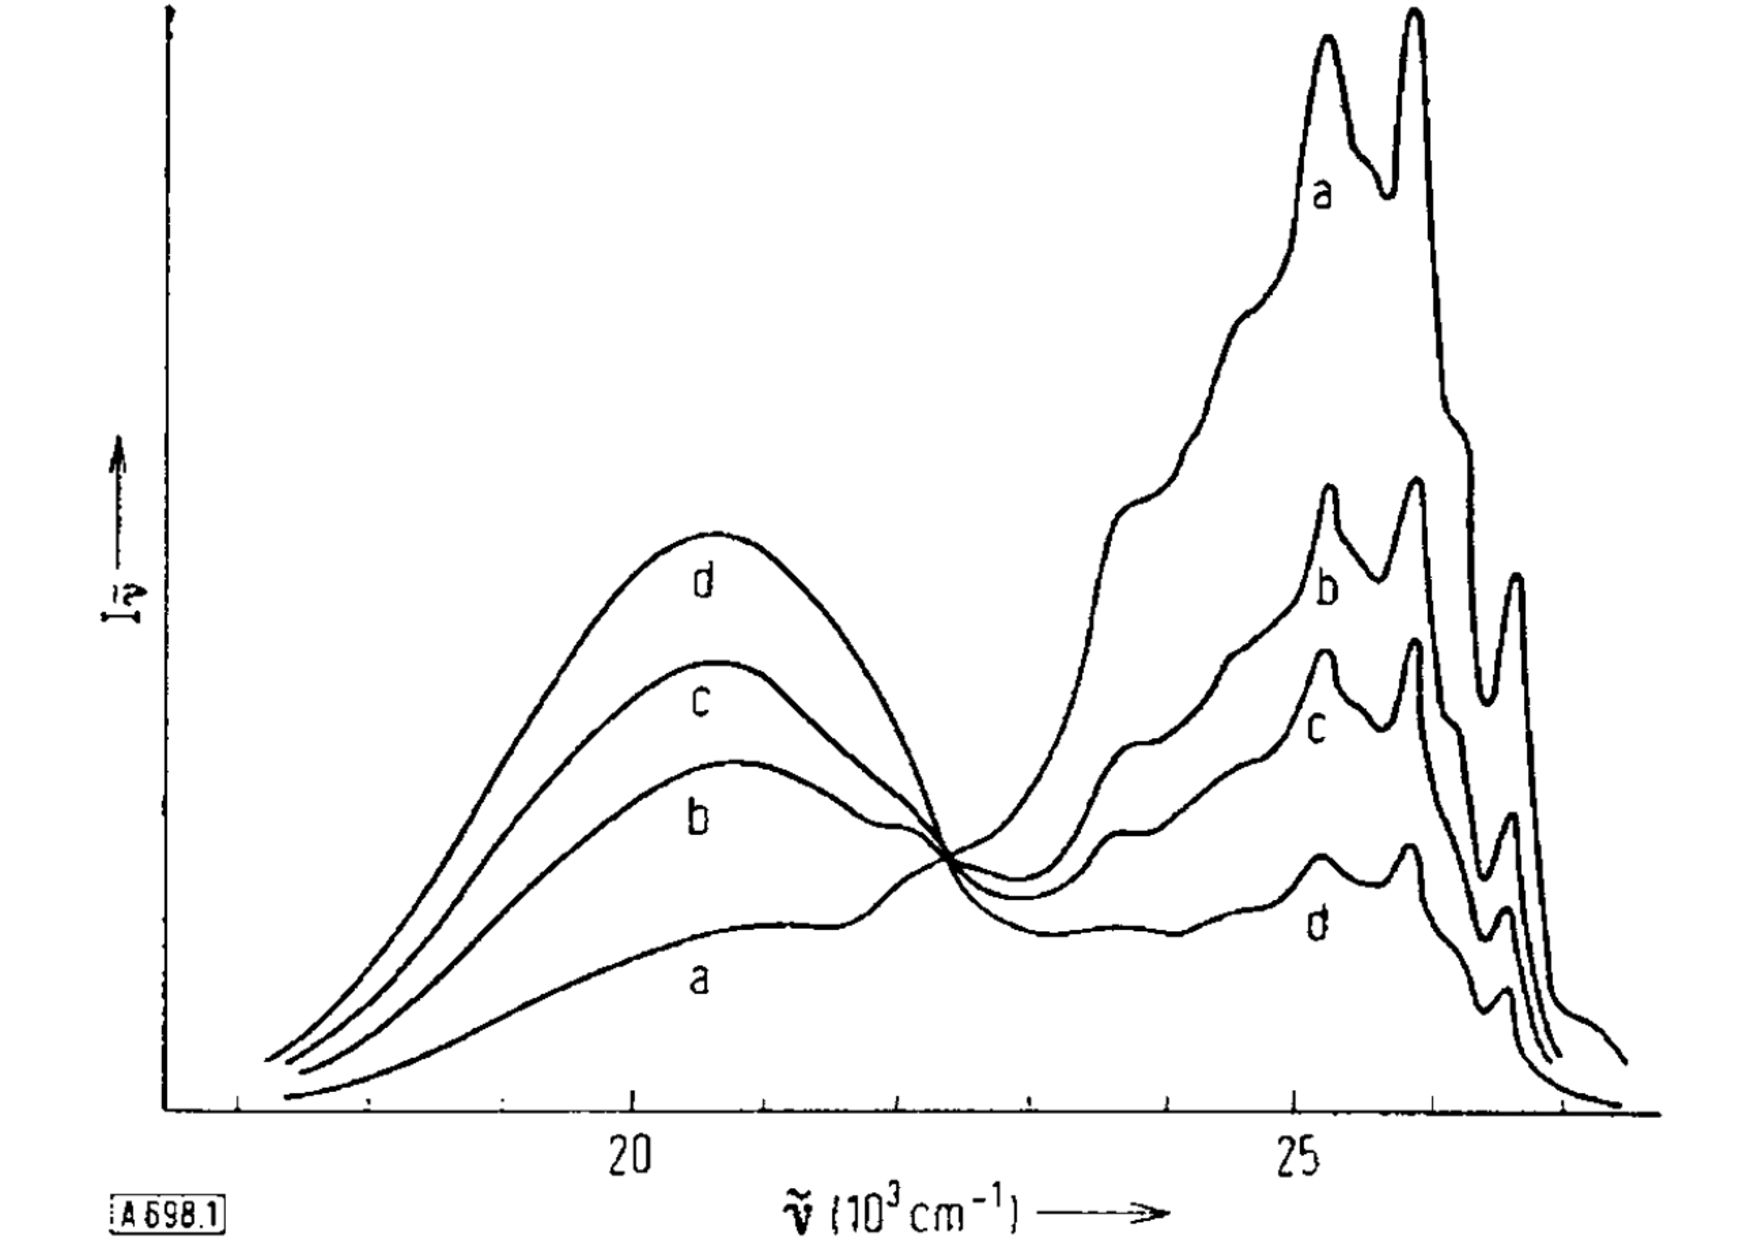
\includegraphics[width=0.6\linewidth]{Intro/Forster_Spectra.pdf}
  \caption[Fluorescence spectrum of pyrene]{Fluorescence spectrum of pyrene (in n-heptane, 20\degree{}C) at different concentrations: a) \SI{5.0e-5}, b) \SI{1.8e-4}, c) \SI{3.1e-4}, d) \SI{7.0e-4}{mol L^{-1}}. Reprinted from ref.~\citenum{Forster1969} with permission of Wiley-VCH.}
  \label{figure: Forster_Spectra}
\end{figure}
This intermolecular phenomenon is detrimental to solid-state fluorescence, and yet is a direct consequence of the design requirements of the chromophore. In biosensing applications, researchers resorted to using dilute solutions with reduced sensitivity because of ACQ.\cite{Thomas2007,Kwok2015} In the solid state, for instance in thin films for optoelectronics, the ACQ effect means that solution screening for viable candidates is rendered meaningless by the differing luminescent properties of the final material compared to the molecule. Strategies to circumvent ACQ have seen varying success, for example through the inclusion of bulky substituents, polar groups, and promotion of hydrogen bonding.\cite{Hong2009,Zhang2013,Mei2014,Mei2015} However, synthetic modification this can in turn effect the chromophore electronic structure and its excited state properties, thus commencing tedious a trail-and-error optimisation process. Attempts to physically block aggregation by encapsulating in surfactants or polymer matrices require extensive engineering and can reduce charge transport.\cite{Hong2009,Chen2000,Lee2013} The deleterious effects of ACQ cannot be underestimated and posed a significant problem for organic luminescent applications. Then, in 2001, the group of Ben Zhong Tang found a system which turned the field on its head and opened a new strategy for the design and development of brightly luminescent organic materials. They named the phenomenon aggregation induced emission (AIE). In the next section of this chapter, the roots of AIE shall be examined, followed by a review of theoretical studies and the subsequent proposed mechanisms.
%%%%%%%%%%%%%%%%%%%%%%%%%%%%%%
\section{Aggregation Induced Emission}\label{section: lom AIE}

